%!TEX program = xelatex
% Note: this template must be compiled with XeLaTeX rather than PDFLaTeX
% due to the custom fonts used. The line above should ensure this happens
% automatically, but if it doesn't, your LaTeX editor should have a simple toggle
% to switch to using XeLaTeX.

\documentclass[
  aspectratio=169, % Uncomment to use an aspect ratio of 16:9 (160 mm by 90 mm)
  %aspectratio=43, % Uncomment to use an aspect ratio of 4:3 (128mm by 96mm)
  t, % Top align all slide content by default
  onlytextwidth, % Typeset content in columns at text width
  10pt, % Default font size, use 10pt for the 16:9 aspect ratio and 8pt for the 4:3 aspect ratio
]{beamer}

\usepackage{../../ImperialTheme/beamer/beamerthemeImperial} % Use the Imperial theme

\def\imagefolder{../../ImperialTheme/beamer/Images}
\def\Rey{\text{Re}}
\title{Instabilities in Quasi-3d} % Presentation title to appear on the title slide and left footers

\subtitle{} % Presentation subtitle to appear on the title slide

\author{Víctor Ballester} % Author name(s) to appear on the title slide

\date{\today} % Presentation date to appear on the title slide and right footers

\begin{document}

\begingroup
\setbeamercolor{background canvas}{bg=ICLLightGrey} % Slide background color
\setbeamercolor{title page title}{fg=ICLBlue} % Title text color
\setbeamercolor{title page subtitle}{fg=ICLBlue} % Subtitle text color
\setbeamercolor{author}{fg=ICLBlue} % Author(s) text color
\setbeamercolor{date}{fg=ICLBlue} % Date text color
\setbeamertemplate{title page}[logo]{\imagefolder/ICL_Logo_Blue.pdf} % Imperial logo color, use 'ICL_Logo_White.pdf' for white and 'ICL_Logo_Blue.pdf' for blue
\frame[plain, s]{\titlepage} % Output the title page with no footer ('plain') and vertically distributed text ('s')
\endgroup


\begin{frame}
  \frametitle{quasi 3d incNS}
	\begin{itemize}
	  \item I tried $L_z = 2d, 3d, 4d$ so far, where $d$ is the gap depth in the gap with $d = 3$ and $w=25$ (just before the Hopf bifurcation in 2d).
	\end{itemize}
\end{frame}
\begin{frame}
  \frametitle{Quasi 3d with $L_z = 2d$ (and also $L_z = 3d$, although I need to double check)}
    \begin{itemize}
      \item Unstable complex mode:
      \item $\sigma = 0.0047955, \omega = 0.0010237$
      \item $v$ component profile:
    \end{itemize}

    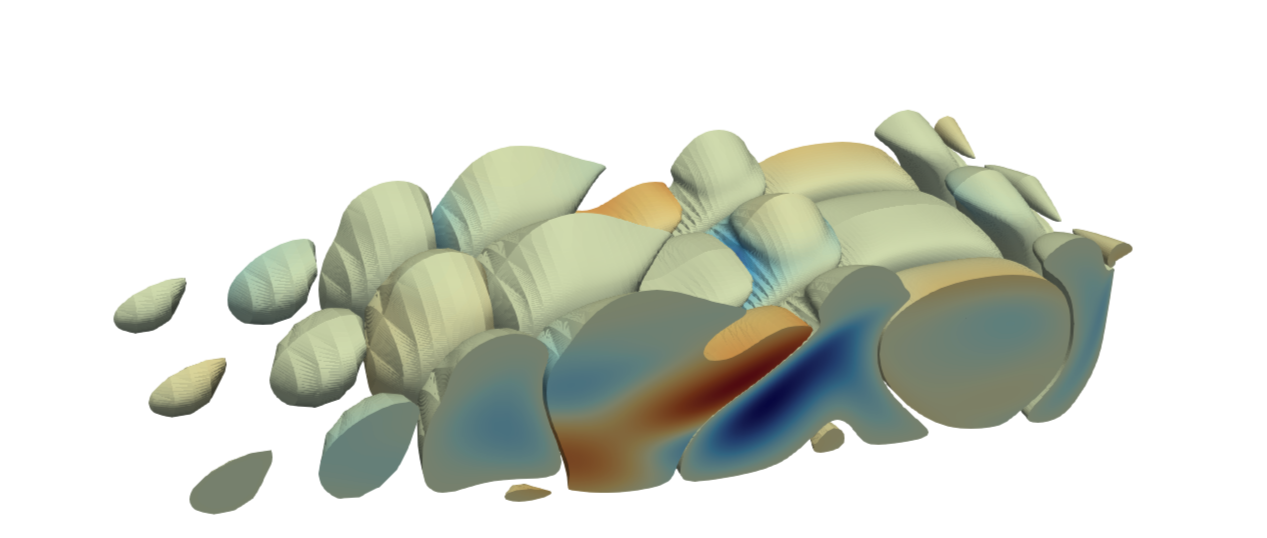
\includegraphics[width=0.8\linewidth]{Images/gapCavityMode.png}
\end{frame}
\begin{frame}
  \frametitle{Quasi 3d with $L_z = 4d$}
\begin{columns}[T] % [T] ensures correct vertical alignment
		\begin{column}{0.49\linewidth} % Left column
		  \begin{itemize}
		    \item The non convergence of the eigenmodes to the same growth rate as we change the integration time between arnoldi iterations is because I think the structure is very long (so more time is needed).

		    \item $\sigma \sim 0.003$ (less than the cavity mode)
		    \item $v$ component profile:
		  \end{itemize}
		\end{column}
		\begin{column}{0.49\linewidth} % Left column
		      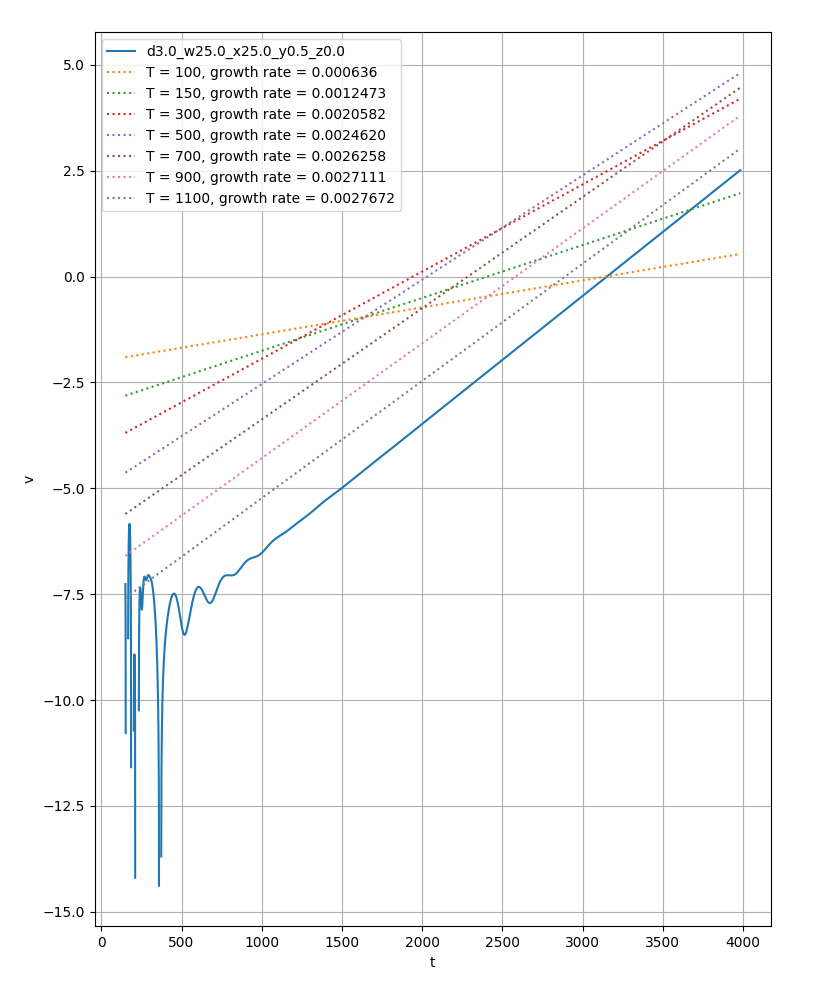
\includegraphics[width=0.88\linewidth]{Images/growthRate.png}
		\end{column}
	\end{columns}
\end{frame}
\begin{frame}
  \frametitle{Marcello Paper 2d stability curve}
	\centering
	\begin{columns}[T] % [T] ensures correct vertical alignment
		\begin{column}{0.49\linewidth} % Left column
		      Ma = 0.5 (Marcello paper):\\
		      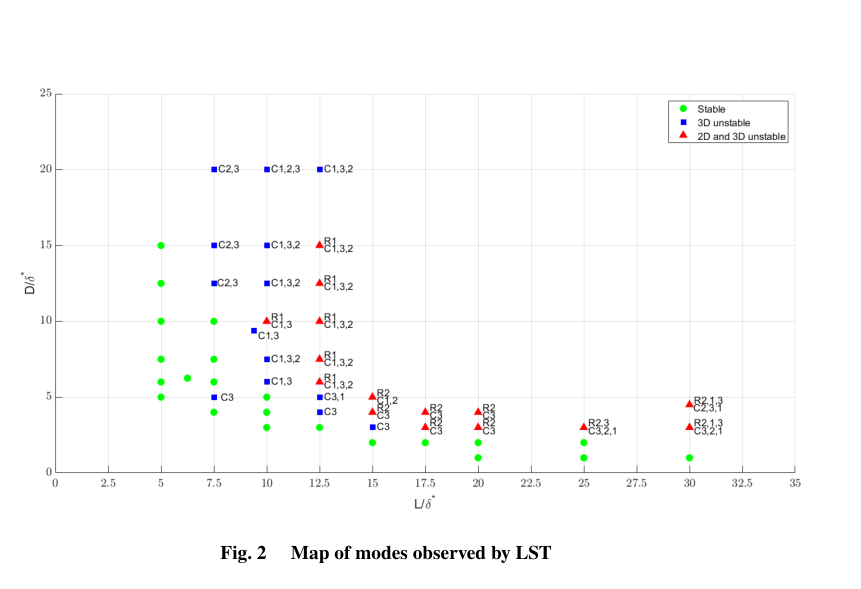
\includegraphics[width=\linewidth]{Images/marcello.png}
		\end{column}
		\begin{column}{0.49\linewidth} % Left column
		      Incompressible case:\\	      
			\includegraphics[width=\linewidth]{../../Images/incNS2dStabilityCurve.pdf}
		\end{column}
	\end{columns}
\end{frame}
\begin{frame}
  \frametitle{d = 3, w = 10 (Ma = 0.6)}
   
  
\includegraphics[width=0.8\linewidth]{Images/d3w10Ma0.6.png}
\end{frame}
\begin{frame}
  \frametitle{d = 1.5, w = 30 (Ma = 0.6)}
  
  
\includegraphics[width=\linewidth]{Images/d1.5w30Ma0.6.png}
\end{frame}
\begin{frame}
  \frametitle{d = 1.25, w = 60 (Ma = 0.6)}
  
  
\includegraphics[width=\linewidth]{Images/d1.25w60Ma0.6.png}

\end{frame}
\end{document}
